\documentclass{article}

\usepackage{graphicx}
\usepackage{pdfpages}
\usepackage{amsmath}
\usepackage{amsfonts}
\usepackage{amssymb}
\usepackage{centernot}
\usepackage{verbatim}
\usepackage{graphicx}
\usepackage[colorlinks]{hyperref}
\usepackage{caption}
\usepackage{subcaption}
\usepackage{titlesec}
\usepackage{scrextend}
\usepackage{titlepic}
\usepackage{float}
\usepackage{wrapfig}
\usepackage{lscape}
\usepackage{rotating}
\usepackage{epstopdf}
\usepackage{pdflscape}
\usepackage[margin=1.2in]{geometry}


\title{\textbf{Catalyst Network - Technical White Paper (DRAFT - V1)}}
\date{\today}
\author{Joseph Kearney\thanks{joseph.kearney@atlascity.io} - Atlas City}


\begin{document}

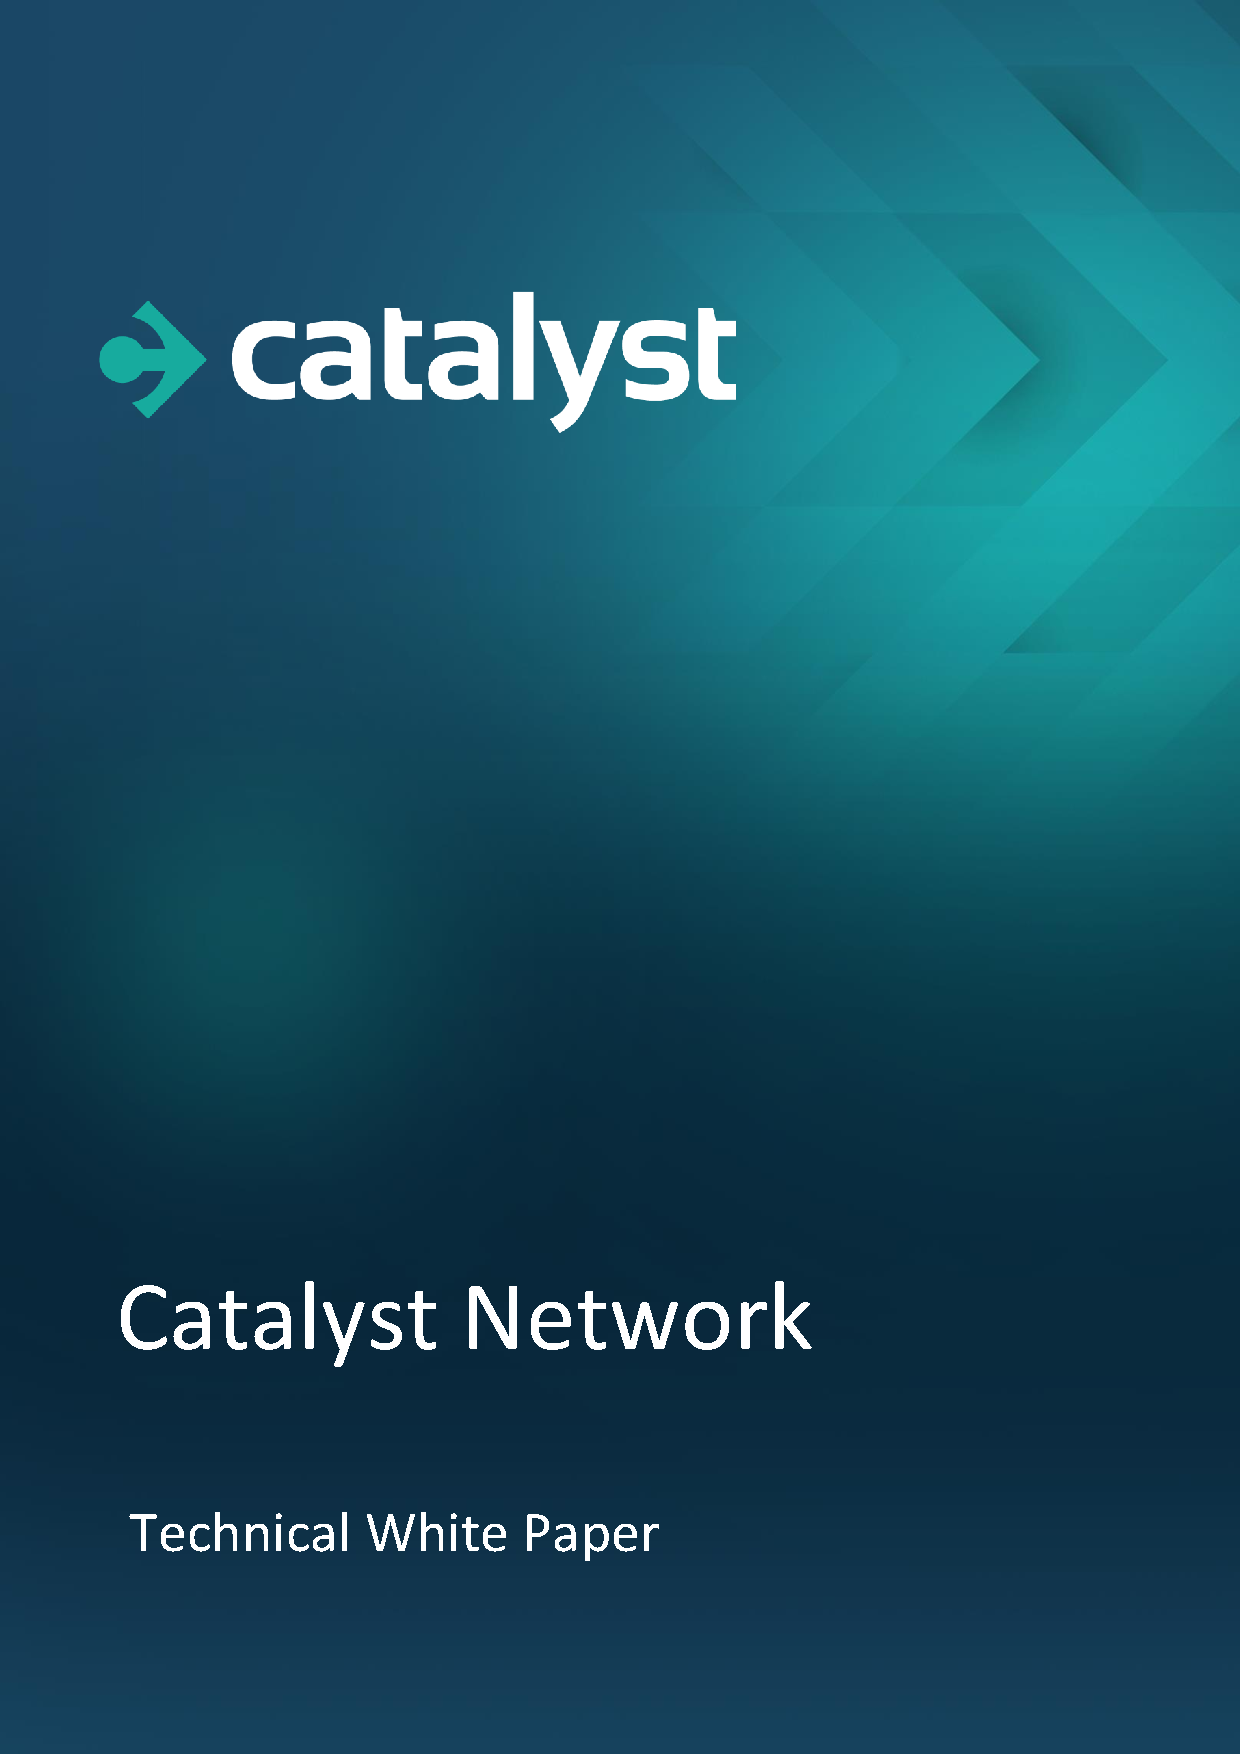
\includepdf [fitpaper=true] {cover-image}

\maketitle

\abstract

Distributed Ledger Technologies (DLTs) over the last decade have grown at an extraordinary rate, with new technologies being announced, developed and released on a daily basis. A majority of these technologies have not progressed from the original concepts set out by Satoshi Nakamoto in his seminal paper \cite{nakamoto2008bitcoin} with regards to speed, security, scalability and decentralisation. There has however been a clear demonstration for the appetite and innovation for wider markets to adopt these technologies. Catalyst marries together many existing technologies as well as some novel ones in order to create a framework which give a fast, scalable and fair ledger.

\begin{center}
\vspace{50mm}
\textbf{This document is a work in progress and is subject to change.}
\end{center}

\newpage

{
  \hypersetup{linkcolor=black}
  \tableofcontents
}
\newpage

\section*{Introduction}

DLTs are based upon the principle of a truly distributed network, allowing nodes on the network to transact both messages and objects. Whether that be tokens, messages, timestamps or even rich file types. Distributed networks have many advantages over centralised systems, particularly the prevention of any one entity from holding too much influence within a system thereby allowing them to perform unfair or malicious acts, furthermore they allow trustless transactions, meaning that you do not have to trust a single person on the network, rather trust the network as a whole. However, for these advantages there are also many problems to overcome, particularly how do you fairly and efficiently ensure consensus among the network is reached, how are the file stored without causing the network to become extremely bloated and also how do you compute complex business logic across a network as efficiently if not more so than on a centralised network. These are all problems that have been considered in the design process of Catalyst. \\

The first problem described was ensuring a fair consensus mechanism. The network coming to agreement on what transactions on a distributed network are fair and valid and those that are not are is a key issue. Early blockchain and DLTs utilised proof of work, this originates from hashcash \cite{back2002hashcash}, which was designed as a prevention mechanism for email spam. This idea was then developed for the bitcoin blockchain, it required miners to perform a computationally hard problem in order for them to expend energy and there by resources. This dissuades mining nodes from acting maliciously, as both the transactions they have added as well as the work they have performed can be verified. If their work is poor then the block they are trying to append to the blockchain will be rejected. This technique for consensus is Byzantine fault tolerant and can not be understated as the critical factor that allowed blockchain technologies to grow. However, this has two critical flaws, firstly the amount of expended and wasted energy is extraordinary especially on large networks where the potential rewards are large \\




The technologies discussed in this paper are:

\begin{itemize}
\item The Distributed File System (DFS) - Catalyst integrates a distributed file system meaning that there is a separation between the ledger and what is stored on the ledger.
\item The Kat Virtual Machine (KVM) - Based upon the innovative Ethereum Virtual Machine (EVM), the KVM improves and extends on the EVM. It allows smart contracts to be run on Catalyst.
\item The Probabilistic Byzantine Fault Tolerant (PBFT) consensus algorithm. This new consensus algorithm allows a fair and scalable mechanism for consensus and updates to the ledger to be agreed upon.
\end{itemize}



\section{Distributed File System}

Catalyst integrates its own Distributed File System (DFS) \cite{DFS} based on the InterPlanetary File System (IPFS) protocol \cite{benet2014ipfs}. DFS as the name suggests are peer to peer file systems, where the files contained within are distributed across a range of peers (and thereby accessible to those peers). This file system unlike others that rely on centralized servers will have no down time nor are a single point of failure, meaning that they are persistent in a way that other file storage technologies are not. \\

On the Catalyst network every node holds a DFS module. This means that while all nodes will not hold all the information stored of the DFS they will be able to query and retrieve information that is of value to them. Furthermore, nodes will simply have the ability to query the existence of a file rather than being forced to download the file in order to check
its existence. \\

Integrating DFS allows the Catalyst network to remain lean as nodes on the network can choose to store only the data that they choose to hold. Furthermore, it allows the storage of many rich file types in a distributed manor, meaning that they are always accessible with no down time guaranteed. In this section is a description of the IPFS platform that Catalyst uses, and then how Catalyst integrates this into its ecosystem.


\subsection{IPFS}

The InterPlanetary File System forms the basis of the Catalyst DFS. IPFS is simply a file system, this can be used to store retrieve and distribute files to other peers. It is itself based on a distributed network, meaning that there is no one central entity that holds and controls the flow of information. \\

An advantage that IPFS has compared to traditional computer filing systems where the URL or file path describe its location, on IPFS what is contained in the file is declared, this is called content addressing, this is using a Content Identifier (CID). This CID is a hash of the contents of the file, thereby changing the contents would change the hash and thereby the CID. Through content addressing, a malicious entity would not be able to send a user a false file in the place of the on that they have requested. This is due to the hardness of reversing a hashing function.\\

Once a file has a CID associated with it a distributed hash table can be formed. Distributed hash tables are key-value stores, which which the elements are held as hashes. The CID becomes the key element. Any peers that hold the file have their ID's associated with the file.  \\

IPFS integrates Merkle Directed Acyclic Graphs (Merkle DAGs). Merkle DAGs are used to form linkages between blocks of information. For example if an entire folder is added to IPFS, the entire folder would have a CID, but additionally the constituent elements would also. The leaf nodes would be formed of the constituent files.


\subsection{Integrating the DFS}

Each node on the running on the catalyst network must also be running the DFS module. This allows them on the most basic level to access the current state of the ledger and the validate previous updates to the ledger thereby allowing them to sync with the current ledger state. \\

The primary difference between the native IPFS protocol and the implementation utilised on Catalyst is how the peer ID's are created.  While on the IPFS protocol the identifier for nodes is selected randomly, on Catalyst the nodes on the network will each have their own individual peer identifier\cite{BytesExtentions} made up of:

\begin{itemize}
\item IP address
\item Port number
\item Public key
\end{itemize}



\subsection{The Marketplace}

\section{KVM}

The Catalyst network \cite{KVM}

The first problem described was ensuring a fair consensus mechanism. The network coming to agreement on what transactions on a distributed network are fair and valid and those that are not are is a key issue. Early blockchain and DLTs utilised proof of work, this originates from hashcash \cite{back2002hashcash}, which was designed as a prevention mechanism for email spam. This idea was then developed for the bitcoin blockchain, it required miners to perform a computationally hard problem in order for them to expend energy and there by resources. This dissuades mining nodes from acting maliciously, as both the transactions they have added as well as the work they have performed can be verified. If there work is poor then the block they are trying to append to the blockchain will be rejected. This technique for consensus is Byzantine fault tolerant and can not be understated as the critical factor that has allowed blockchain technologies to grow. However, this has two critical flaws, firstly the amount of expended and wasted energy is extraordinary especially on large networks where the potential rewards are large. Secondly there has been a general trend towards centralisation at scale, as mining pools hold increase their share of the network power (and thereby the networks rewards) \\

The second issue considered while building the Catalyst network is how bloating on the network is avoided. Running a full node on many blockchains requires a significant amount of disk space, for example the Ethereum blockchain size has exceeded 1Tb \cite{EthBloat} and continues to grow. Catalyst solves this problem through the integration of a Distributed File System (DFS). This enables much more control for peers on the network what elements of the ledger that they hold. This means lightweight nodes can be ran. Furthermore, large data files can be securely held on the ledger without causing issues for other nodes due to bloating. \\

The final issue Catalyst aims to solve is the ability for complex business logic and smart contract to be ran on the ledger. While smart contracts are capable of being ran on a wide variety of blockchains frequently they are simple and incapable of running complex solutions. Often also requiring a user to write smart contracts in a specialised language. \\


\section{Catalyst Consensus Mechanism}

On distributed networks there is no single point of trust to determine the validity of transactions, therefore concurrency must be ensured by other methods. Typically this requires a majority of the network's participants to agree on a particular update of the ledger and the account balances / holdings held within. Blockchain technologies generally employ Proof-of-Work (PoW) and occasionally Proof-of-Stake (PoS) mechanisms in order to gain consensus across a network. However, these methods are prone to increasing centralization at scale as well as in the case of PoW high energy consumption. Other networks employ a small amount of trusted nodes that ensure the validity of transactions, however this is highly centralised and almost as fallible as the single point of failure systems that DLT endeavors to avoid. \\

Catalyst integrates a newly designed consensus mechanism, based on Probabilistic Byzantine Fault Tolerance (PBFT).  This is a collaborative rather than competitive protocol, meaning that all honest work performed by nodes on the network benefits the security of the network and that all participating nodes are rewarded equally. For each ledger cycle a random selection of worker nodes are selected, the nodes become the producers for a cycle or number of cycles. The producer nodes perform work in the form of compiling and validating transaction thereby extracting a ledger state change for that cycle. \\


The protocol is split into four distinct phases:

\begin{itemize}

\item Construction Phase - Producer nodes that have been selected create what they believe to be the correct update of the ledger. They then distribute this proposed ledger update in the form of it hash digest.
\item Campaigning Phase - Producer nodes designate and declare what they believe to be the most popular ledger state update.
\item Voting Phase -
\item Synchronisation Phase - In this phase the producers who have computed the correct ledger update can broadcast this update the rest of the network.

\end{itemize}

This section is based on the work set out in \cite{catalystresearch}, where the original research into the creation of a new consensus mechanism are laid out.

\subsection{Notation}

\subsection{Producer Node Selection}



Original work for the Catalyst consensus mechanism states that the peers are selected with relation to the PID and the hash of the previous data. As the PID can be manipulated by a user and thereby weight in their favor of selection to become a producer this is not usable. \\

Research into a RANDAO provides a viable alternative \cite{skvorc}\cite{randao}. Generation of a process by which each user creates their own random value and then by combining these random numbers across the network you gain distributed generated pseudo-random numbers. The larger the network the more random the number will be. The proposed process works as follows: \\

\begin{itemize}

\item Each node $n$ in the worker pool $N$ generates a random number $r$.
\item To this random number the hash of the previous ledger state, $D$, must be added.
\item $n$ then creates a Blake-2b hash of the combined random number $H(r + D)$.
\item Each $n$ must then send their value $r$ to the contract.
\item If they do not send their $r$ value they are not eligible to become a producer node.
\item Each $n$ in $N$ sends their $H(r + D)$ to a hard coded smart contract. This creates the global random value $R$. This is done through addition of all the random numbers.
\item The smart contract must determine:
\begin{itemize}
\item Whether $n$ did submit all correct information. i.e. $r$, and $H(r+D)$.
\item That $n$ did in fact use the $D$ value when generating the random number. This is done by taking the $r$ value submitted by the user and hashing with $D$.
\item Ensuring $n$ has paid a sufficient stake to take part in the selection process.
\item Validating that each worker $n$ has only distributed one random number to the smart contract.
\end{itemize}
\item Failure of any one of these points means the smart contract will not accept the submission of a random number from $r$ and and stake made will be lost.
\item This global random can the be used to determine the producers for the next cycle(s).
\item This is done by determining the nodes that have a $H(r + D)$ closest to the $R$ value. \\

\end{itemize}


This method is secure from manipulation as hashing algorithms are one way functions meaning that there is no provably efficient method to inverse a hashing function i.e. retrieving a message $m$ from a digest $H(m)$. If a node does not input a value into the smart contract then they are not eligible for selection for becoming a producer for that cycle(s). \\

Addition of the $D$ value is necessary as this will prevent a producer from using known random values to create a desired digest that gives them an advantage when being selected. The value for $D$ must fulfill two rules, firstly it must always be the same for all nodes in the worker pool, secondly it must change with each draw of a random number when determining the random selection of producer nodes. This prevents a user creating a hash using known input and digest combinations to gain an advantage when being selected. Furthermore if the hash of the previous ledger state is used as $D$ is ensures that a prospective producer node knows the current ledger state. If they do not then their random number will be invalid as $H(r + D_{prod}) \neq H(r + D)$. \\

As described in RANDAO, this can be further extended to implement staking. Nominal fees to contribute can be added in order to prevent DDOS. This is done in such a way that a nominal fee is added as to not dissuade users from legitimately wanting to become producers while dissuading malicious entities from attempting to perform a Sybil attack against the network in order to gain majority control over a producer pool for a cycle or multiple cycle. There is also the additional benefit of simplification of the overall consensus mechanism as it removes the need for a queuing mechanism as well as producing a verifiable method of keeping track of what nodes are registering to be workers for any given cycle. It also thereby in turn provides evidence to other nodes on the network who the producers for any given cycle are as the process will be verifiable. \\

This scheme will provide the Catalyst consensus mechanism with a verifiable, reliable and secure mechanism to generate a pool of producers. By randomly assigning which workers get to participate in the next ledger cycle, fairness is ensured. \\



%%%%%%%%%%%%%%%%%%%%%%%%%%%%%%%%%%%%%%%%%%%%%%%%%%%%%%%%%%%%%%%%%%%%%%%%%%%%%%%%%%

\subsection{Notation} 

A dictionary for the variables used in the proceeding description of the consensus mechanism can now be described for clarity:

\begin{itemize}

\item $p$ - Describes a single producer that has been selected randomly to perform work for the network for a given cycle. 
\item $P$ - The pool of producers who have been selected through the previously described producer selection mechanism for the particular cycle being described. It is made up of a set of producers $p$
\item $T$ - The mempool of any given producer $p$. It contains a group of transactions that will be used to for the update for a given cycle. 
\item $t$ - A single transaction that is found within the mempool $T$. 
\item $u$ - The local ledger state update generated by a single producer node. This is what that particular node believes to be the correct update for the given cycle. 
\item $\sigma$ - A pseudorandomly generated number. 
\item $E$ - The list of entries found within a single transaction $t$. A producer will producer  will producer one of these lists for each valid transaction in $T$.
\item $d$ - Hash tree containing all the signatures extracted from the transactions in $T$.
\item $H$ - Hash of each list $E$ combined with the salt $\sigma$.
\item $L$ - Alphanumerically ordered list the pair $E,H$, sorted according to $H$. 
\item $G$ - The list of proposed updates $u$ that producer $p$ collects from other nodes in producer pool $P$. This is used to determine the most popular update. 
\item $\mathcal{L}(prod)$ - The list of producers from a particular producers set $G$ that sent the most popular ledger state update.
\item $L_{CE}$ - A producers list of compensation entries i.e. who a producer believes did the correct work for the network and thereby should be rewarded. 
\item $\mathcal{L}(vote)$ - The list of producers a specific producer found to have forwarded the correct vote for the most popular ledger state update. 
\item $LSU$ - Ledger State Update, this is the final ledger state update proposed by a producer node. It consists of the list of entries used to create the update, the hash tree containing the signatures and the list of compensation entries
\item $V$ - A producers vote for the correct $LSU$ formed of the hash of the LSU, $L_{vote}$ and the producers Id.

 

\end{itemize}

\subsection{Construction Phase}

The first phase of the Catalyst consensus algorithm is the Construction Phase. Within which the selected producer nodes  $P$ calculate their proposed ledger state update or their local ledger state update. This is done by aggregating and validating all transactions that have occurred during a set time period. These transactions assuming their validity are integrated into the producers local ledger state update. From which they can create a hash of the update. This hash digest represents what they believe to be the correct update and is broadcast to the other producer nodes during for that cycle. Assuming the collision free nature of hash functions, the only mechanism for multiple producer nodes to have the same local ledger state update is by both using the same set of transactions. \\



Each producer $p$ in the set of producers $P$ follows the same protocol. The construction phase begins with producer $p$ beginning their construction phase by flushing their mempool. This mempool $T$ is made up of $n$ transactions $t$  where $n$ is the number of transactions that have been broadcast to the network and have been stored by $p$. These transaction are used to create $p$'s local ledger state update $u$.  \\

The producer at this point also creates a hash trees $d$, this is to store the the signatures that are extracted from each transaction in $T$. A salt $\sigma$ is created utilizing a pseudo-random number generator using the previous ledger state update $U-1$ as its seed. $p$ then follows the following steps:

\begin{enumerate}
\item Producer $p$ verifies that each transaction in $T$ is valid following the rules set out in \cite{transactionvalidator}. From each of the $n$ transactions in $T$ the entries $E$ that constitute the transaction $t$ are extracted to form a list $E = e_1,...,e_m$ for $m$ entries in $t$. The producer should therefore end up with $n$ lists for $E$ from $T$. each signature from the transactions are also extracted and added to $d$.

\item $p$ for each $E$ it created then creates a corresponding hash digest as:
\begin{center}
$H = \mathcal{H}[E~||~\sigma]$
\end{center}

Each pair ($E,O$) is added to a list $L$.

\item $p$ then sorts list $L$ into lexicographical order according the hash values $H$.

\item The producer $p$ then extracts the transaction fee value from each transaction in $T$ to create $v$ which is the total sum of all transaction fees.

\item The local ledger state update $u$ for producer $p$ can then be calculated. Firstly the list $L$ is concatenated (denoted by $||$) with the hashtree $d$ and a hash digest is created as:

\begin{center}
$u = \mathcal{H}(L~||~d)$
\end{center}

$u$ is then concatenated with $p$'s unique peer identifier $Id$ to create:

\begin{center}
$h = u ~||~Id$
\end{center}

\item $h$ is then broadcast to the other producer nodes on the network.
\end{enumerate}



Producer $p$ also collects other producers partial ledger update values. At most they will collect $P-1$ values. Optimally every producer in $P$ will receive the same set of transactions therefore for every $p$ in $P$ will have the same partial ledger update $u$. However this is unlikely due to all transactions not being received by a small group of nodes. Equally they may not hold $G$ where $G = h_1,...,h_P$, meaning they may not receive a proposed update from all candidates.

%%%%%%%%%%%%%%%%%%%%%%%%%%%%%%%%%%%%%%%%%%%%%%%%%%%%%%%%%%%%%%%%%%%%%%%%%%%%%%%%%%%

\subsection{Campaigning Phase}

The second phase of the consensus mechanism is where producer $p$ generates and proposes a candidate, which it calculates to be the most popular ledger state update. \\


Beginning this phase producer $p$ has a set of partial ledger updates $G$ that it has received from other producer nodes. Each $h$ within $G$ contains a producers hash of the proposed update ($u$ and a peer identifier ($Id$). The most popular $u$ value can be found, this gives us $u^{maj}$ from there the subset $G_{maj}$ can be created, which is the amount of votes for the most popular update. Two thresholds must be considered first is $G_{min}$ this is the minimum amount of updates it has received from other producers in order to generate a valid candidate. The second is $G_{thresh}$ this is the threshold value for which a minimum number of votes must be in favor of $G_{maj}$ which the most popular vote found within $G$.  So in order to proceed with declaring a candidate $G > G_{min}$ and $G_{maj} > G_{thresh}$. \\

Beginning this phase producer $p$ has a set of partial ledger updates $G$ that it has received from other producer nodes. Each $h$ within $G$ contains a producers hash of the proposed update ($u$ and a peer identifier ($Id$). The most popular $u$ value can be found, this gives us $u^{maj}$ from there the subset $G_{maj}$ can be created, which is the amount of votes for the most popular update. Two thresholds must be considered first is $G_{min}$ this is the minimum amount of updates it has received from other producers in order to generate a valid candidate. The second is $G_{thresh}$ this is the threshold value for which a minimum number of votes must be in favor of $G_{maj}$ which the most popular vote found within $G$.  So in order to proceed with declaring a candidate $G > G_{min}$ and $G_{maj} > G_{thresh}$. \\

If the thresholds are met the following can take place:

\begin{enumerate}
\item $p$ creates a list $\mathcal{L}(prod)$. To this list $p$ appends the identifier of any producer that correctly sent the $u$ value that equals $u^{maj}$. If $p$'s $u$ value is also the same as $u^{maj}$ then they should append their own $Id$.
\item Producer $p$ then creates their candidate for the ledger update $c$ which is calculated as $c = u^{maj}~||~\#(\mathcal{L}(prod))~||~Id$
\item Producer $p$ will then broadcast their preferred update $c$ to the other producers.
\end{enumerate}




$p$ during this phase will be collecting the $c$ values from other producers. At the end of this phase of the cycle $p$ will hold a set of $C$ candidates.


%%%%%%%%%%%%%%%%%%%%%%%%%%%%%%%%%%%%%%%%%%%%%%%%%%%%%%%%%%%%%%%%%%%%%%%%%%%%%

\subsection{Voting Phase}

The third phase of the ledger cycle is the Voting Phase within which a producer $p$ from the $C$ candidates it has received decides on what it believes should be the global ledger state update i.e. the update that should be applied to the ledger for that cycle.



\begin{enumerate}
\item $p$ verifies that the same first hash value $u^{maj}$ is embedded in a majority of producer candidates.
\item $p$ is required at this point to have created the majority ledger update. As only with this partial update can they participate effectively. Therefore their $u == u^{maj}$

\end{enumerate}

If each producer collects the first hash value generated by every producer, any two producers would build the same list of identifiers $\mathcal{L}(prod)$. However even in highly efficient distributed network it is unlikely that all producers will retrieve all information. Therefore it must be assumed that the list of identifiers held by $p$ is incomplete, $p$ however must ensure that they hold enough information to confidently issue a vote on the update to the ledger. The identifier of a producer is appended to the hash they distribute because:

\begin{itemize}
\item To verify that $p$ is a producer node and that they in fact were one of the winners of the random draw described in \ref{insert ref}.
\item To evaluate and track the quality of the work performed by $p$.
\item To ensure that the correct producers withing $P$ are rewarded for their work maintaining the ledger. \\

\end{itemize}

New transaction entries (compensation entries) are created using the list's  $\mathcal{L}(prod)$ produced by the producers $p$. This allows reward and fees to be paid to the correct users. These new transaction entries will be appended to the final ledger state update for that cycle. Therefore a complete ledger state update should consist of:

\begin{itemize}
\item The list of transaction entries integrated into the new ledger state all $E$ lists.
\item The transaction signatures from $T$ held in $d$.
\item Compensation entries rewarding the producers from $\mathcal{L}(prod)$.

\end{itemize}

The voting process thereby must confirm the correct list of identifiers involved in producing the correct ledger state updates. The final list for  $\mathcal{L}(prod)$ is generated by merging the producers lists together. In order for a producer $p$ to have their $Id$ added to the final  $\mathcal{L}(prod)$ the must appear in at least 50\% of the  $\mathcal{L}(prod)$ lists distributed by $P$. This ensures that no producer can just append their own $Id$ to their update whether that update was correct or not and gain a reward for it.  \\

As explained below the final list $\mathcal{L}_n(prod)$ is obtained by merging the partial lists included in the producers' candidate. A producer $P_j$ could have produced a first hash value $h_{\Delta j}$ different to $h^{maj}_{\Delta j}$ yet added his identifier to $\mathcal{L}_j(prod)$ when building its candidate $c_j$ in the attempt to collect some token reward. In such scenario $Id_j$ would be an element of the list included in $c_j$ (or any other producer node controlled by $P_j$), but it wouldn't be included in any other list $\{\mathcal{L}_k(prod)\} \forall~k \in P/j$. To prevent such malicious behavior, a rule imposes that $P_j$ only appends to the final list $\mathcal{L}_n(prod)$ the identifier of a producer included in the list $\mathcal{L}_k(prod)$ of a candidate $c_k$ satisfying $h^{maj}_{\Delta k} = h^{maj}$ if and only if that identifier is included in at least $P/2$ lists $\{\mathcal{L}_{k}(prod)\}_{k=1,..,V_j}$ associated to a candidate $c_{k}$ satisfying $h^{maj}_{\Delta k} = h^{maj}$. Only a producer controlling half or more of the producer nodes would succeed in including its identifier into the final list $\mathcal{L}_n(prod)$.\\

Although this eliminates the risk of unethical behavior from the producer, this also means that there would be little incentive for a producer to broadcast its vote if its identifier was not included in $\mathcal{L}_n(prod)$. However, the probability that a producer compiles the correct final list $\mathcal{L}_n(prod)$ strongly depends on the number of votes collected. The more votes collected by a producer, the greater the probability that said producer will compile the complete final list. Although a producer may not have produced the correct partial ledger state update, participating in the voting process is, therefore, an important contribution to the overall consensus protocol and should entitle the producer nodes to some reward. To that end a producer $P_j$ can use the identifier of other producers included in their vote and create a second list $\mathcal{L}_j(vote)$ to account for their participation in the voting process. \\

$p$ follows a series of steps:

\begin{enumerate}
\item $p$ generates a list $\mathcal{L}(vote)$ it then appends the $Id$ of any other $p$ that has forwarded a $C$ candidate that satisfies $u == u^{maj}$.
\item $p$ creates the combined list for $\mathcal{L}(prod)$ of any $p$ from $P$ that appears in $P/2$ lists.
\item Then $p$ creates a list $L_{CE}$. This contains the contribution entries. This is for any user that is included in the combined $\mathcal{L}(prod)$. Each of these producers contained within this list will receive $x$ tokens. If it is considered that $X$ is the total number of tokens that are injected into the network at each cycle for the pool of $P$ producers. The amount of entries into $L_{CE}$ will be less than or equal to $P$. $R$ is to be considered the total amount of reward that is to be split among all the producers that found the correct ledger update $R = f_{prod}X + v$ where $f_prod$ is the fraction of the injected tokens that are given to users found in the combined $L_{prod}$. While $(1-f_{prod})X$ is the value that is distributed to other nodes that have performed work.
\item Producer $p$ can then create the candidate ledger state update for this cycle. This includes the reward allocations for producers according to their contributions. This ledger state update $LSU$ can be defined as:

\begin{center}
$\mathbf{LSU = L~||~d~||~L_{CE}}$
\end{center}


$p$ then computes its vote (or \textit{producer vote}):
\begin{center}
\fbox{$V = \mathcal{H}(LSU)~||~\#(\mathcal{L}(vote))~||~Id$}
\end{center}


\item $p$ then forwards their $V$ to the other producers and collects the producer votes $V$ issued by its peers.

\end{enumerate}


\subsubsection{Ballot collection}
During the voting phase, the producer $p$ collects the producer votes $V$ broadcast by its peers. At the end of the voting phase , the producer $p$ holds $U$ producer votes $V$ in its cache. This will be equal to or less than the number of producers who formed the correct update.

During the voting phase, the producer $p$ collects the producer votes $V$ broadcast by its peers. At the end of the voting phase , the producer $p$ holds $U$ producer votes $V$ in its cache. This will be equal to or less than the number of producers who formed the correct update. 

\subsection{Synchronisation Phase}

\subsubsection{Final ledger state update generation and broadcast}



During the synchronisation phase $p$ executes the following steps:

\begin{enumerate}
\item $p$ defines the ledger state update $\Delta L_n$ for the cycle $\mathcal{C}_n$ as:\\
 $\mathcal{H}(\Delta L_n) = max[unique(\mathcal{H}(LSU_k))~\forall~k\in\{U_j\}]$ and the associated number of votes collected: $U^{maj} = count[(\mathcal{H}(LSU_k) = \mathcal{H}(\Delta L_n))~\forall~k\in\{U_j\}]$ and verifies that $U^{maj}> U_{threshold}$.
\item $P_j$ creates a new list $\mathcal{L}_{n}(vote)$ and append to $\mathcal{L}_{n}(vote)$ the identifier of a producer included in the list $\mathcal{L}_{k}(vote)$ of a vote $v_k$ satisfying $\mathcal{H}(LSU_k) = \mathcal{H}(\Delta L_n)$ if and only if the identifier is included in at least $C_n/2$ lists $\{\mathcal{L}_{k}(vote)\}$ associated to a producer vote $v_{k}$ satisfying $\mathcal{H}(LSU_k) = \mathcal{H}(\Delta L_n)$. Note that $C_n$ can be easily computed as it corresponds to the number of producer identifiers who correctly computed the ledger state update and are therefore included in $\mathcal{L}_{n}(prod)$.

\item If $P_j$ generated the correct ledger state update $\Delta L_n$, it can write it to DFS which will return it with a content-based address $\mathcal{A}_n$.
\item A Producer $P_j$ then creates the following output quantity (or \textit{producer output}):
\begin{equation}
\fbox{$\mathbf{o_{j} = \mathcal{A}_n~||~\#(\mathcal{L}_{n}(vote))~||~Id_j}$}
\label{eq:Hj}
\end{equation}
The producer then broadcasts $o_j$ to the network.
\end{enumerate}


\subsubsection{Ledger state synchronisation across the network}

During the time period [$t_{s}, t_s + \Delta t_{cycle}$], user nodes collect $\{o_k\}_{\forall k \in P}$ producer outputs broadcast by the producers.
By extracting the identifier $Id_k$ embedded in any collected output $o_k$, a user node can easily compile a list of producer identifiers having broadcast the same second hash value $\mathcal{H}(\Delta L_n)$ (concatenated with the same list $\mathcal{L}_{n}(vote)$). Upon receiving $x > P/2$ identical addresses $\{\mathcal{A}_k = \mathcal{A}_n\}_{k \in x}$, the user nodes can read the common address content ($\Delta L_n$) from DFS. Using $\Delta L_n$ a user node can safely synchronise their local copy of the ledger and write it to their DFS if not already done. The balance of accounts stored on the ledger are updated and the producers effectively collect their rewards.\\


Worker nodes also store the list $\mathcal{L}_{n}(vote)$ embedded in each $o_k$ output. If selected to be a producer for the next cycle $\mathcal{C}_{n+1}$, a worker can use it to generate the reward allocated to the producers who correctly voted for the accurate ledger state update during the ledger cycle $\mathcal{C}_{n}$.\\


The various parameters and thresholds mentioned in this chapter and their impact on the levels of security and confidence in the successful production of a ledger state update are discussed in the paper found here \cite{catalystresearch2}.

\section{Distributed File System}

Catalyst integrates its own Distributed File System (DFS) \cite{DFS} based on the InterPlanetary File System (IPFS) protocol \cite{benet2014ipfs}. DFS as the name suggests are peer to peer file systems, where the files contained within are distributed across a range of peers (and thereby accessible to those peers). This file system unlike others that rely on centralized servers will have no down time nor are a single point of failure, meaning that they are persistent in a way that other file storage technologies are not. \\



On the Catalyst network every node holds a DFS module. This means that while all nodes will not hold all the information stored of the DFS they will be able to query and retrieve information that is of value to them. Furthermore, nodes will simply have the ability to query the existence of a file rather than being forced to download the file in order to check
its existence. \\                                                                                                                                                                                                                                                                                                                                                                                                                                                                                                                                                                                                                                                                                                                                                                                                                                                                                                                                                                                                                                                                                                                                                       

Integrating DFS allows the Catalyst network to remain lean as nodes on the network can choose to store only the data that they choose to hold. Furthermore, it allows the storage of many rich file types in a distributed manor, meaning that they are always accessible with no down time guaranteed. In this section is a description of the IPFS platform that Catalyst uses, and then how Catalyst integrates this into its ecosystem. 


\subsection{IPFS}

The InterPlanetary File System forms the basis of the Catalyst DFS. IPFS is simply a file system, this can be used to store retrieve and distribute files to other peers. It is itself based on a distributed network, meaning that there is no one central entity that holds and controls the flow of information. Across the IPFS network nodes hold as little or as much data as the wish with multiple copies of the data being held across many unrelated nodes. This means that there is no single point of failure in the network. An attempted attack on the IPFS would require a majority of nodes to be taken offline to prevent access to the files held on the network.   \\

IPFS uses a bittorrent style \\

An advantage that IPFS has compared to traditional computer filing systems where the URL or file path describe its location, on IPFS what is contained in the file is declared, this is called content addressing, this is using a Content Identifier (CID). This CID is a hash of the contents of the file, thereby changing the contents would change the hash and thereby the CID. Through content addressing, a malicious entity would not be able to send a user a false file in the place of the on that they have requested. This is due to the hardness of reversing a hashing function. The CID also means that all files stored on IPFS are immutable i.e. can not be edited as changing anything contained within the file means that that CID for that file will now be changed. Through linkage of these files it means that a version history of files can be created. \\

Once a file has a CID associated with it a distributed hash table can be formed. Distributed hash tables are key-value stores, which which the elements are held as hashes. The CID becomes the key element. Any peers that hold the file have their ID's associated with the file. The CID associated with a file means that the file is not duplicated on the network. For example if Alice uploads file $x$ it is stored on IPFS, other users can then download and hold the file, if then Bob uploads the same file $x$ then because the CID for both files would be the same the duplication would not take place as the file is already held on the file system.  \\

IPFS integrates Merkle Directed Acyclic Graphs (Merkle DAGs). Merkle DAGs are used to form linkages between blocks of information. For example if an entire folder is added to IPFS, the entire folder would have a CID, but additionally the constituent elements would also. The leaf nodes would be formed of the constituent files. Merkle DAG's are used compared to traditional Merkle trees as the allow a flow or direction of information to be established. Thereby allowing an order for the reading of the files to be set. 


\subsection{Integrating the DFS}

Each node on the running on the catalyst network must also be running the DFS module. This allows them on the most basic level to access the current state of the ledger and the validate previous updates to the ledger thereby allowing them to sync with the current ledger state. This is required as it is necessary for the all nodes on the network at the very least to know the current state of the ledger in order to send transactions. \\

The primary difference between the native IPFS protocol and the implementation utilised on Catalyst is how the peer ID's are created.  While on the IPFS protocol the identifier for nodes is selected randomly, on Catalyst the nodes on the network will each have their own individual peer identifier\cite{BytesExtentions} made up of:

\begin{itemize}
\item IP address
\item Port number
\item Public key
\end{itemize}

This allows user to be able to identify who on the network is holding specific files as each peer identifier for a node will be unique. This means that a peer on the network will have a clear target for where they can retrieve given information, furthermore it means that nodes claiming to hold specific files and information are accountable for being able to distribute these files. Through the use of Catalyst peer identifiers within the DHTs peers can make informed decisions on who they retrieve files from, for example if a node has been marked as malicious due to actions within the network, they will also not be trusted within the DFS.


\subsection{The Marketplace}

\textbf{WIP} \\



\section{KVM}

\textbf{WIP} \\

The Catalyst network integrates and improves upon the Ethereum Virtual Machine (EVM) to create the Kat Virtual Machine (KVM) \cite{KVM}. This allows complex smart contracts to be run on Catalyst, as well allowing pre-existing smart contracts written in Solidity to be used on Catalyst. By extending the rand of Op-Codes that are used on the EVM, we can ensure that significantly more complex operations can be performed.

\subsection{From the EVM}

EVM is the run-time environment that enables smart contracts on the Ethereum blockchain. It relies on the fact that when a smart contract is ran upon two different machine using the same inputs both machines will retrieve the same output i.e. it is deterministic. Smart contracts can be written primarily in the Solidity language.

\subsection{To the KVM}

As EVM requires smart contract developers to write in Solidity this can prove to be restrictive. The KVM allows smart contracts to be able to write smart contracts in a wide variety of languages. 






\section*{Conclusion}

Through the use of the technologies described

Futher information on Catalyst and its applications can be found at: \\
\begin{center}
Atlas City website - \url{https://www.atlascity.io/} \\
Catalyst website - \url{https://www.catalystnet.org/}\\
Catalyst GitHub - \url{https://www.github.com/catalyst-network}\\
\end{center}



\bibliography{catalyst-technical-whitepaper}
\bibliographystyle{ieeetr}

\end{document}